Apache Openwhisk is an \textbf{open-source serverless} platform created by \textbf{IBM} that executes functions in response to events, scaling automatically and managing all necessary infrastructure and services. OpenWhisk competes with large platforms like \textit{Nginx}, \textit{Kafka}, \textit{Docker}, and \textit{CouchDB}; together, these tools help create a comprehensive serverless cloud service.\vspace{14pt}\\
It’s commonly used for applications that need \textbf{flexibility}, \textbf{scalability}, and \textbf{agility}, especially where real-time processing or dynamic scaling is important. Some pratical scenarios where Openwhisk shines are \textit{Real-Time Data Processing}, \textit{IoT Data Processing}, \textit{Automated DevOps Tasks} and \textit{Serverless API Backend}.\vspace{14pt}\\
Additionally, OpenWhisk provides a \textit{Command Line Interface} (\textit{CLI}), known as \textbf{wsk}, which allows developers to easily create, execute, and manage OpenWhisk entities across any operating system, making platform interactions straightforward for developers.\vspace{14pt}\\
Apache Openwhisk supports flexible deployment options across various platforms due to its containerized components, which enable deployment both locally and within cloud infrastructures. It can be deployed on platforms such as \textit{Kubernetes}, \textit{Mesos}, and \textit{OpenShift}.\vspace{14pt}\\
The programming model of Apache Openwhisk is built around three core components:\\
\textit{Actions}, \textit{Triggers}, and \textit{Rules}.\vspace{14pt}\\
\textbf{Actions} are stateless functions that execute arbitrary code; \textbf{Triggers} represent a class of events originating from various sources, and \textbf{Rules} link a Trigger to an Action. OpenWhisk also allows chaining Actions into sequences.\vspace{14pt}\\
The model supports multiple programming languages, including \textit{Java}, \textit{Python}, and \textit{JavaScript}, and uses an event-driven architecture where most \textbf{Actions execute in response to events}.\cite{quevedo2019evaluating}\vspace{10pt}
\begin{center}
    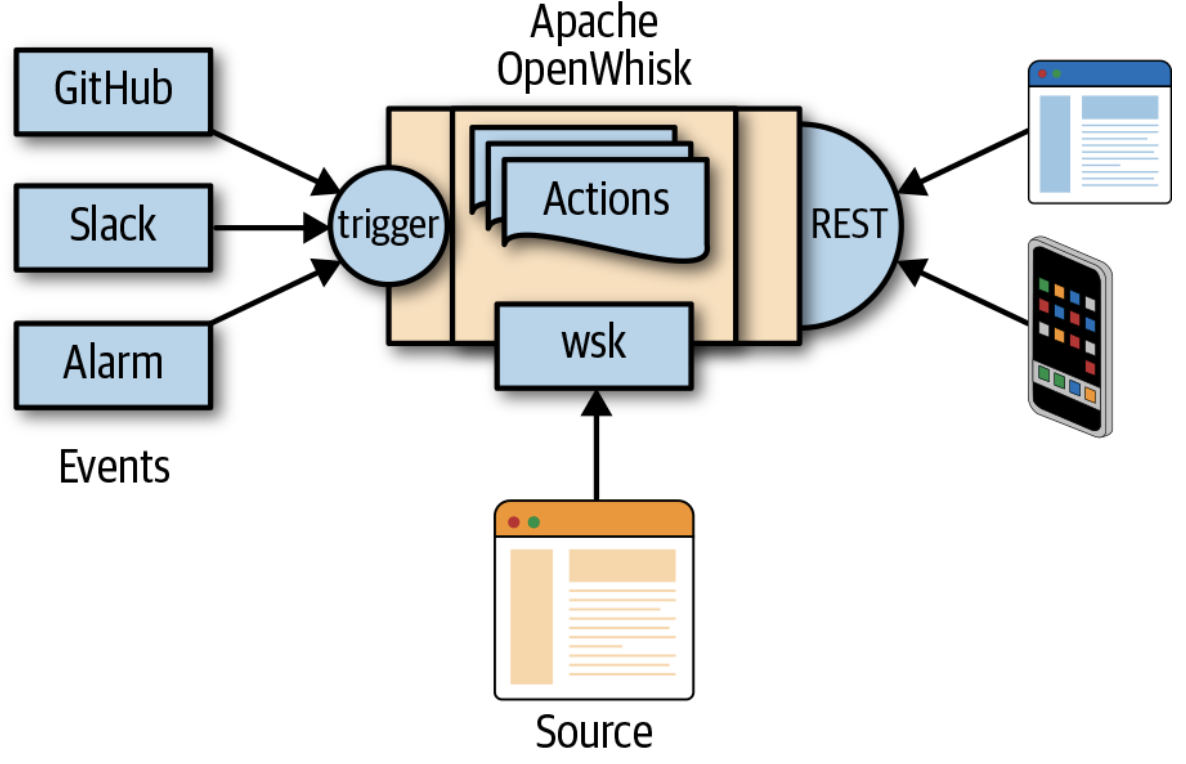
\includegraphics[width=0.7\textwidth]{img/ow_works.png}
    \captionof{figure}{How Apache Openwhisk works}
    \vspace{10pt}
\end{center}
In summary, this platform’s key features include\cite{huy2021crypto}:
\begin{itemize}
    \item \textbf{Deploys Anywhere}: with its container-based architecture, Apache Openwhisk offers versatile deployment options, supporting both local setups and various cloud infrastructures.
    \item \textbf{Supports Any Programming Language}: OpenWhisk is compatible with a wide range of programming languages, including NodeJS, Java, Scala, PHP, Python, and others. For unsupported platforms or languages, users can easily create and customize executables using Docker SDK to run on Docker.
    \item \textbf{Integration Support}: OpenWhisk enables easy integration of developed Actions with popular services through pre-built packages, either from independent projects or the default catalog. These packages offer integrations with services such as Kafka message queues, databases, mobile applications, messaging services, and RSS feeds.
    \item \textbf{Rich Function Composition}: functions written in multiple programming languages can be packaged with Docker for flexible invocation options, including synchronous, asynchronous, or scheduled execution. Parameter binding is recommended to prevent hardcoding service credentials directly into code.
    \item \textbf{Scalability and Resource Optimization}: OpenWhisk allows Actions to scale instantly, handling thousands of executions in seconds or running only as needed, such as on a weekly schedule. Resources scale automatically to match demand, pausing when idle, so users only pay for actual usage with no costs for unused resources.
\end{itemize}